\documentclass[runningheads]{llncs}

\usepackage[T1]{fontenc}
\usepackage{graphicx}
\usepackage{hyperref}

% If you use the hyperref package, please uncomment the following two lines
% to display URLs in blue roman font according to Springer's eBook style:
\usepackage{color}
\renewcommand\UrlFont{\color{blue}\rmfamily}
\urlstyle{rm}

%----Making things more compact
\newcommand{\smalltt}[1]{\small \texttt{#1}}
\newenvironment{packed_itemize}{
\vspace*{-0.2em}
\begin{itemize}
\setlength{\partopsep}{0pt}
\setlength{\itemsep}{1pt}
\setlength{\parskip}{0pt}
\setlength{\parsep}{0pt}
}{\end{itemize}}
\newenvironment{packed_enumerate}{
\vspace*{-0.2em}
\begin{enumerate}
\setlength{\partopsep}{0pt}
\setlength{\itemsep}{1pt}
\setlength{\parskip}{0pt}
\setlength{\parsep}{0pt}
}{\end{enumerate}}
\renewcommand{\textfraction}{0.07}
\renewcommand{\topfraction}{0.9}
\renewcommand{\bottomfraction}{0.9}
\renewcommand{\floatpagefraction}{0.66}
\setlength{\floatsep}{2.0pt plus 2.0pt minus 2.0pt}
\setlength{\textfloatsep}{5.0pt plus 2.0pt minus 0.0pt}
\title{SUMO-NLP-LLM: A Neuro-Symbolic Question Answering System}
\titlerunning{SUMO-NLP-LLM}
\author{
Adam Pease\inst{1}\orcidID{0000-0001-9772-1266} \and
Roberto Milanese\inst{1}\orcidID{0009-0009-5107-162X} \and
Jarrad Singley\inst{1}\orcidID{1111-2222-3333-4444} \and
Richard Thompson\inst{1}\orcidID{0009-0001-6541-1092} \and
Angelos Toutisios\inst{1}\orcidID{0009-0009-6064-5154} \and
Geoff Sutcliffe\inst{2}\orcidID{0000-0001-9120-3927}}

\authorrunning{A. Pease et al.}

\institute{Naval Postgraduate School, Monterey, USA \\
\email{\{adam.pease,roberto.milanese,jarrad.singley,richard.thompson,angelos.toutsios.gr\}@nps.edu}\\
\and
University of Miami, Miami, USA \\
\email{geoff@cs.miami.edu}}

\begin{document}
\maketitle              % typeset the header of the contribution
%--------------------------------------------------------------------------------------------------
\begin{abstract}
The abstract should briefly summarize the contents of the paper in
150--250 words.

\keywords{First keyword  \and Second keyword \and Another keyword.}
\end{abstract}
%--------------------------------------------------------------------------------------------------
\section{Introduction}
\label{Introduction}

\cite{PB10-IKBET}

\begin{figure}
% 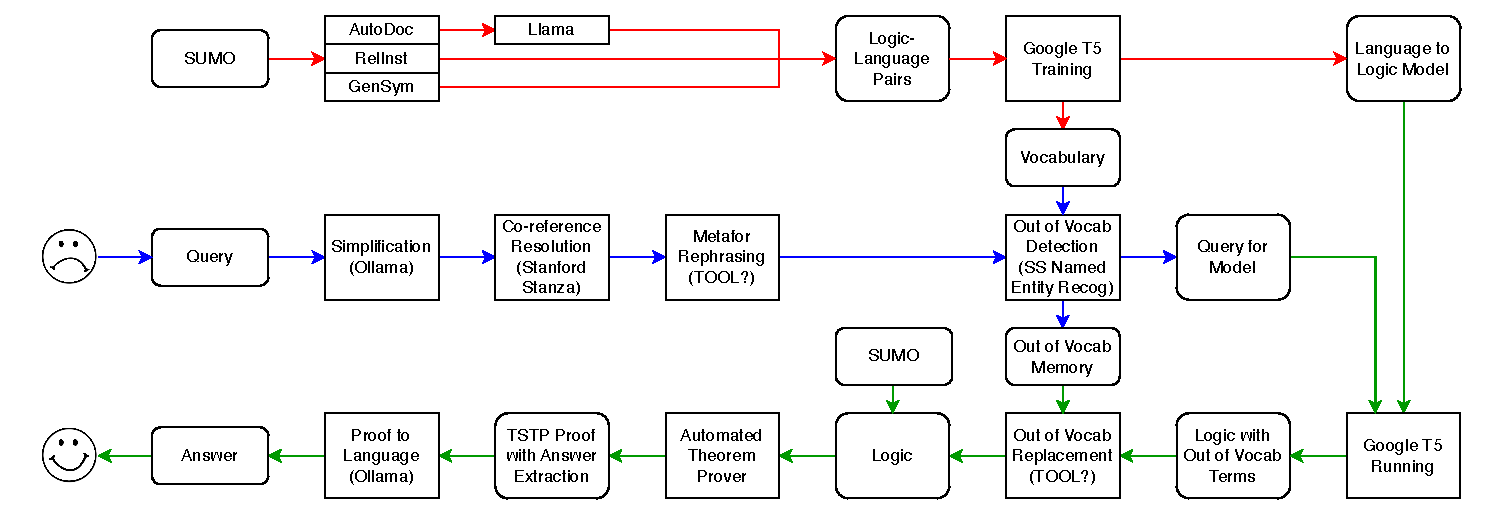
\includegraphics[width=\textwidth]{Architecture.pdf}
\caption{SUMO-NLP architecture}
\label{Architecture}
\end{figure}

%--------------------------------------------------------------------------------------------------
\section{Architecture}
\label{Architecture}

%--------------------------------------------------------------------------------------------------
\section{Training}
\label{Training}

%--------------------------------------------------------------------------------------------------
\section{Running}
\label{Running}

%--------------------------------------------------------------------------------------------------
\section{Conclusion}
\label{Conclusion}

%--------------------------------------------------------------------------------------------------
\bibliographystyle{splncs04}
\bibliography{Bibliography.bib}
%--------------------------------------------------------------------------------------------------
\end{document}
%--------------------------------------------------------------------------------------------------
